\documentclass[12pt]{article}
 
\usepackage{setspace}

\usepackage[LGR,T1]{fontenc} % Support Icelandic Characters
\usepackage[utf8]{inputenc} % Support Icelandic Characters
\usepackage{graphicx} % Support for including images

%\usepackage{hyperref} % Support for hyperlinks

\usepackage[breaklinks]{hyperref}
\hypersetup{colorlinks=true,linkcolor=blue,filecolor=magenta,urlcolor=cyan,unicode=true, pdftitle={Ομάδα 4},bookmarks=true,final=true,}
\urlstyle{same}

\usepackage{wrapfig}
\usepackage{float}
\usepackage{longtable}
\usepackage{array}
\usepackage{subcaption}
\usepackage[left=2.5cm, right=2.5cm, top=2.5cm, bottom=2.5cm, bindingoffset=0.2cm, head=15pt]{geometry}

\usepackage{caption}
\usepackage{mathtools}
\usepackage{bm}
\usepackage{esvect}
\usepackage{titlesec}
\usepackage[autostyle=true]{csquotes}
\titlespacing\section{0pt}{12pt plus 4pt minus 2pt}{0pt plus 2pt minus 2pt}
\titlespacing\subsection{0pt}{12pt plus 4pt minus 2pt}{0pt plus 2pt minus 2pt}
\titlespacing\subsubsection{0pt}{12pt plus 4pt minus 2pt}{0pt plus 2pt minus 2pt}



\usepackage[greek,english]{babel}
\usepackage{alphabeta}
 \newcommand{\lat } {\latintext}

%------------------------------------------------------------------
% TITLE
%------------------------------------------------------------------
\title{
\centerline{
\includegraphics[width=50mm]{images/ekpa.PNG}}
\vspace{0.5 cm}
Εργασία Ομάδας 4\\
\vspace{0.5cm}
\lat{SPS...S}
\large  \\
ΣΤΑΤΙΣΤΙΚΗ ΑΝΑΛΥΣΗ ΔΕΔΟΜΕΝΩΝ \\ 
\vspace{0.5cm}
\small ΔΔΠΜΣ στην Ιατρική Φυσική – Ακτινοφυσική \\
\vspace{0.5cm}
\small Ομάδα 4:\\
\small Βαράκα Μαρία \\
\small Γιαννακούλη Παναγιώτα \\
\small       Γκεζέρης Γιώργος \\
  \small     Τσελεπής Δημήτριος
  }


  

\date{15/12/2019}

\setlength{\parindent}{4em}
\setlength{\parskip}{1em}
%------------------------------------------------------------------
% DOCUMENT START HERE
%------------------------------------------------------------------
\begin{document}
\maketitle

\clearpage
\section*{Περίληψη}
Η παρούσα εργασία αφορά τη στατιστική ανάλυση και επεξεργασία δεδομένων με τη χρήση του στατιστικού υπολογιστικού πακέτου SPSS.

Οι μεταβλητές που χρησιμοποιήθηκαν για τη στατιστική ανάλυση είναι:
\begin{itemize}
  \item Πρώτο καρδιακό επεισόδιο \lat{(nominal)}
  \item Ηλικία \lat{(scale)}
  \item ΔΑΠ-Διαστολική Αρτηριακή Πίεση \lat{(scale)}
  \item Χοληστερόλη \lat{(scale)}
  \item Αριθμός τσιγάρων \lat{(scale)}
  \item Επιβίωση μετά από 10 χρόνια \lat{(nominal)}
  \item Οικογενειακό Ιστορικό ΚΕ \lat{(nominal)}
\end{itemize}

\underline{Για τις κατηγορικές μεταβλητές (nominal)} ως μέτρο θέσης δόθηκε η επικρατούσα τιμή \lat{(Mode)} , ως σχετικά διαγράμματα τα Pie Chart και Histogram καθώς και οι πίνακες συχνοτήτων.

\underline{Για τις ποσοτικές μεταβλητές (scale)} ως μέτρα θέσης δόθηκαν η επικρατούσα τιμή (Mode), η διάμεσος (Median) και η μέση τιμή (Mean) , ως μέτρα διασποράς δόθηκαν η τυπική απόκλιση (St.dev) και η διακύμανση (Variance) , ως μέτρα μορφής δόθηκαν οι συντελεστές κύρτωσης (Coefficient of Kurtosis) και ασυμμετρίας (Coefficient of Skewness), ως σχετικά διαγράμματα τα Histogram και θηκόγραμμα (Box plot).


\clearpage
\section{Περιγραφικές διαδικασίες του \lat{SPSS} (Α) }

Κοιτώντας την τελευταία γραμμή του πίνακα Statistics μπορούμε να δούμε την επικρατούσα τιμή (Mode) για καθεμία από τις υπό μελέτη μεταβλητές (Πρώτο καρδιακό, Επιβίωση μετά από 10 χρόνια, Οικογενειακό ιστορικό ΚΕ). Παρατηρούμε πως για το πρώτο καρδιακό επεισόδιο η επικρατούσα τιμή ισούται με 1, ενώ για τις άλλες δύο κατηγορικές μας μεταβλητές η επικρατούσα τιμή είναι η 0.

Οι υπόλοιποι πίνακες με τίτλους Πρώτο καρδιακό επεισόδιο , Επιβίωση μετά από 10 χρόνια, Οικογενειακό ιστορικό ΚΕ είναι οι πίνακες συχνότητας των αντίστοιχων μεταβλητών, από τους οποίους στη στήλη Frequency βλέπουμε τις συχνότητες εμφάνισης της κάθε κατηγορίας κάθε μεταβλητής. Στη στήλη Valid Percent βλέπουμε τα έγκυρα ποσοστά τα οποία για να υπολογιστούν δεν λαμβάνονται υπόψη οι τιμές που δεν έχουν απαντηθεί \lat{(missing values)}. Σύμφωνα με τον πίνακα Statistics φαίνεται πως δεν υπάρχουν missing values. Η στήλη Cumulative Percent (αθροιστικό ποσοστό) εδώ δεν έχει νόημα, επειδή οι μεταβλητές είναι κατηγορικές.

\begin{figure}[hb]
 \centering
            \begin{subfigure}{0.8\textwidth}
     \centering
         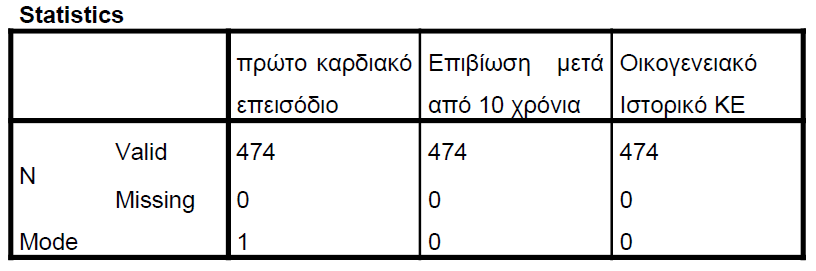
\includegraphics[width=\textwidth]{images/1.PNG}
                      \end{subfigure}
                      
     \begin{subfigure}{0.8\textwidth}
     \centering
         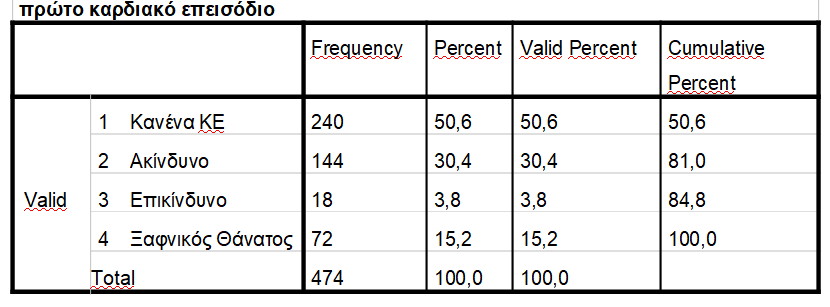
\includegraphics[width=\textwidth]{images/2.PNG}
                      \end{subfigure}
    \end{figure}
    
    \clearpage
    \begin{figure}[ht]
     \centering
     \begin{subfigure}[ht]{0.8\textwidth}
     \centering
         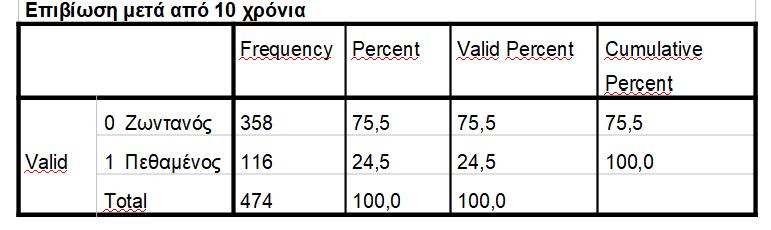
\includegraphics[width=\textwidth]{images/3.PNG}
              \end{subfigure}
     
     \begin{subfigure}[ht]{0.8\textwidth}
     \centering
         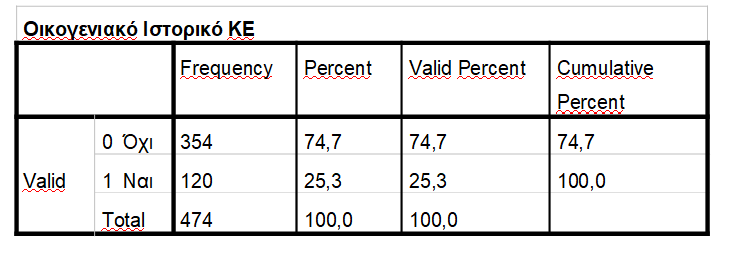
\includegraphics[width=\textwidth]{images/4.PNG}
             \end{subfigure}
      
\end{figure}

Από τους παραπάνω πίνακες παρατηρούμε τα εξής:
\begin{itemize}
    \item Για το πρώτο καρδιακό επεισόδιο η μεταβλητή με τη μεγαλύτερη συχνότητα εμφάνισης είναι η κατηγορία με τον κωδικό 1 = Κανένα ΚΕ και ποσοστό 50,6 \%.
    \item Για την Επιβίωση μετά από 10 χρόνια η μεταβλητή με τη μεγαλύτερη συχνότητα εμφάνισης είναι η κατηγορία με τον κωδικό 0 = Ζωντανός και ποσοστό 75,5 \%.
    \item Για το Οικογενειακό ιστορικό ΚΕ η μεταβλητή με τη μεγαλύτερη συχνότητα εμφάνισης είναι η κατηγορία με τον κωδικό 0 = Όχι και ποσοστό 74,7 \%.
    
\end{itemize}


Τα παραπάνω συμπεράσματα για τις κατηγορικές μεταβλητές επαληθεύονται και από τα ακόλουθα ραβδογράμματα και \lat{Pie charts}.

\clearpage

\begin{figure}[hb]
 \centering
            \begin{subfigure}{0.7\textwidth}
     \centering
         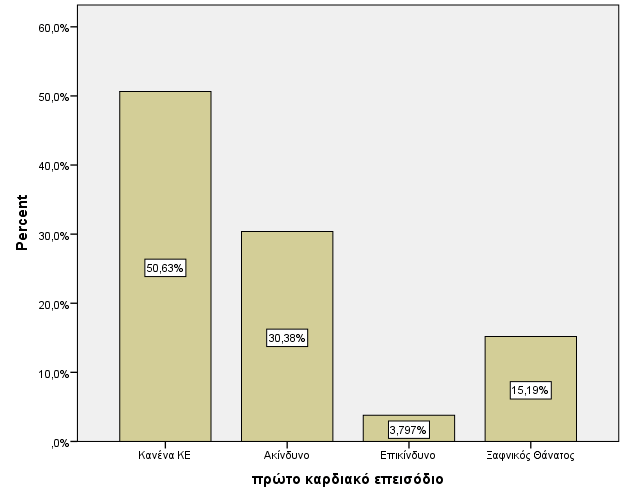
\includegraphics[width=\textwidth]{images/5.png}
                      \end{subfigure}
                       
     \begin{subfigure}{0.6\textwidth}
     \centering
     \vspace{2cm}
         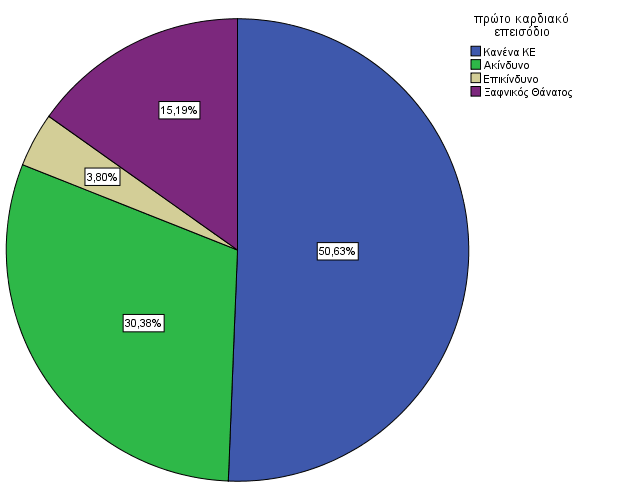
\includegraphics[width=\textwidth]{images/6.png}
                      \end{subfigure}
    \end{figure}

\clearpage
\begin{figure}
 \centering
            \begin{subfigure}{0.7\textwidth}
     \centering
         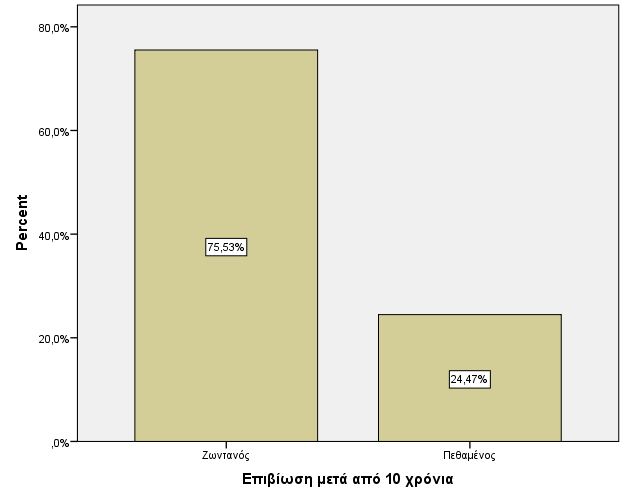
\includegraphics[width=\textwidth]{images/7.png}
                      \end{subfigure}
                      
     \begin{subfigure}{0.6\textwidth}
     \centering
     \vspace{2cm}
         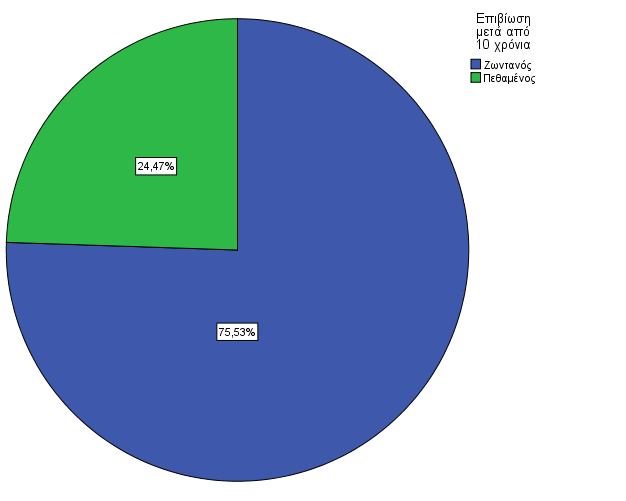
\includegraphics[width=\textwidth]{images/8.png}
                      \end{subfigure}
    \end{figure}
    
    \clearpage
\begin{figure}
 \centering
            \begin{subfigure}{0.7\textwidth}
     \centering
         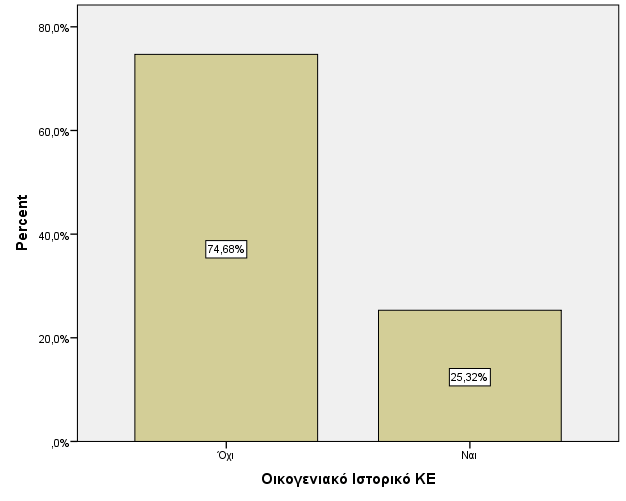
\includegraphics[width=\textwidth]{images/9.png}
                      \end{subfigure}
                      
     \begin{subfigure}{0.6\textwidth}
     \centering
     \vspace{2cm}
         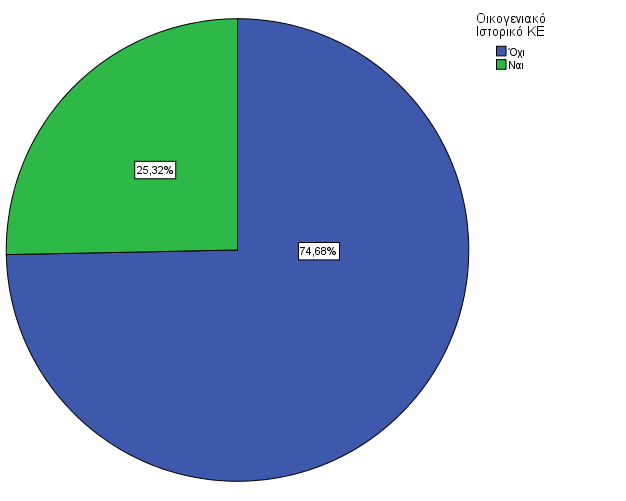
\includegraphics[width=\textwidth]{images/10.png}
                      \end{subfigure}
    \end{figure}
   
   \clearpage 
    Στον ακόλουθο πίνακα παρουσιάζονται όλα τα μέτρα θέσης , διασποράς και μορφής για τις scale μεταβλητές της στατιστικής μας ανάλυσης.
    
    \begin{figure}[hb]
        \centering
        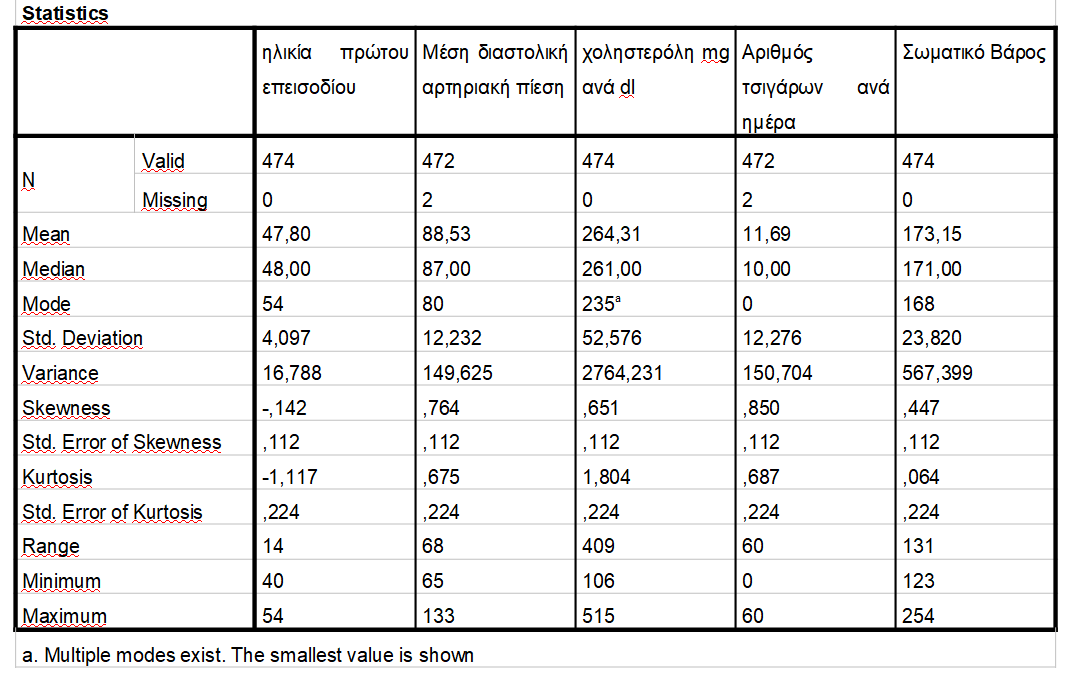
\includegraphics[width=\textwidth]{images/11.PNG}
    \end{figure}
    
    Για τη μεταβλητή ηλικία πρώτου επεισοδίου παρατηρούμε πως ο συντελεστής  skewness είναι αρνητικός (-0,142) , για τη μέση διαστολική αρτηριακή πίεση είναι θετικός (+0,764) όπως και για τη χοληστερόλη (+0,651) , τον αριθμό τσιγάρων ανά ημέρα (+0,850) και το σωματικό βάρος (+0,447) . Όταν ο συγκεκριμένος συντελεστής έχει αρνητική τιμή η κορυφή της κατανομής μετατοπίζεται προς τα δεξιά ενώ όταν έχει θετική τιμή μετατοπίζεται προς τα αριστερά. Επιπλέον η συσσώρευση των παρατηρήσεων προς τα αριστερά ή δεξιά της κατανομής εξετάζεται και μέσω της σύγκρισης των μέτρων της μέσης (mean) και της ενδιάμεσης τιμής (median). Εάν η μέση τιμή είναι μικρότερη της ενδιάμεσης τότε έχουμε αρνητική συμμετρία, ενώ εάν είναι μεγαλύτερη έχουμε θετική συμμετρία, πράγμα το οποίο αποδεικνύεται και από τον πίνακα.

Για τη μεταβλητή ηλικία πρώτου επεισοδίου παρατηρούμε πως ο συντελεστής  kurtosis είναι αρνητικός (-1,117) , για τη μέση διαστολική αρτηριακή πίεση είναι θετικός (+0,675) όπως και για τη χοληστερόλη (+1,804) , τον αριθμό τσιγάρων ανά ημέρα (+0,687) και το σωματικό βάρος (+0,064) . Όταν ο συγκεκριμένος συντελεστής έχει αρνητική τιμή η κατανομή μπορεί να θεωρηθεί πλατύκυρτη, ενώ όταν έχει θετική τιμή μπορεί να θεωρηθεί λεπτόκυρτη.

Σημειώνεται πως οι τιμές των συντελεστών ασυμμετρίας και κύρτωσης πρέπει να βρίσκονται μέσα στο διάστημα -2 έως 2, κάτι το οποίο τηρείται και από τα δεδομένα του πίνακα.


Τα παραπάνω συμπεράσματα για το συντελεστή skewness και kurtosis για τις ποσοτικές μεταβλητές επαληθεύονται και από τα ακόλουθα ιστογράμματα.

\begin{figure}[hb]
 \centering
            \begin{subfigure}{0.65\textwidth}
     \centering
         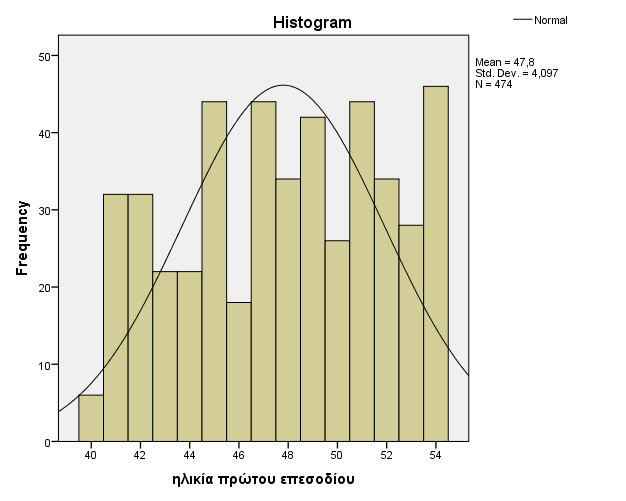
\includegraphics[width=\textwidth]{images/12.png}
                      \end{subfigure}
                     
     \begin{subfigure}{0.65\textwidth}
     \centering
     \vspace{0.5cm}
         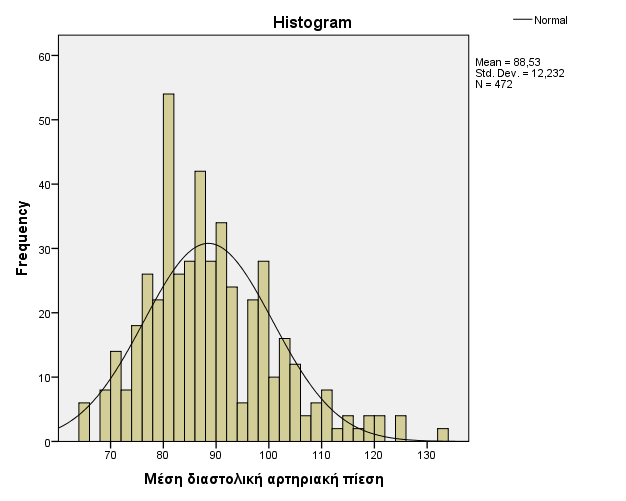
\includegraphics[width=\textwidth]{images/13.png}
                      \end{subfigure}
    \end{figure}
    
    \clearpage
    \begin{figure}
 \centering
            \begin{subfigure}{0.7\textwidth}
     \centering
         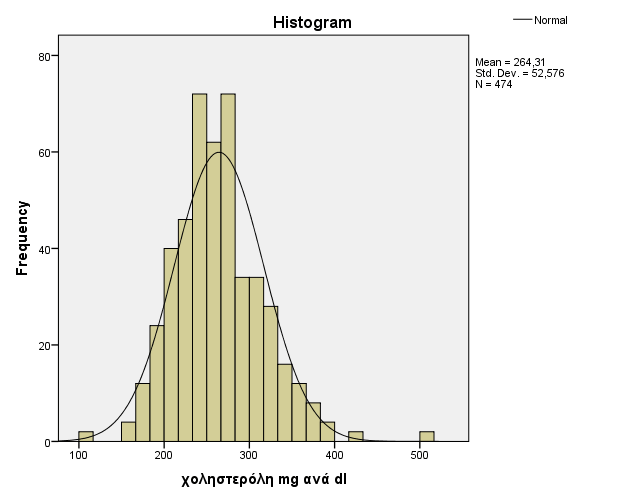
\includegraphics[width=\textwidth]{images/14.png}
                      \end{subfigure}
                      
     \begin{subfigure}{0.7\textwidth}
     \centering
     \vspace{0.5cm}
         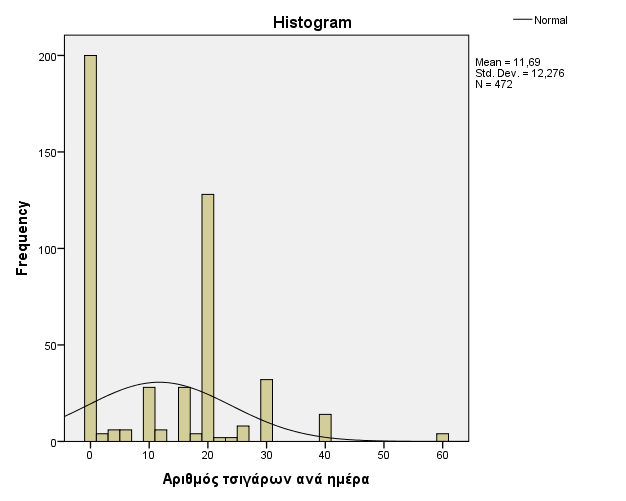
\includegraphics[width=\textwidth]{images/15.png}
                      \end{subfigure}
    \end{figure}
    
    \clearpage
    
    \vspace{0.5cm}
    
    \begin{figure}
        \centering
        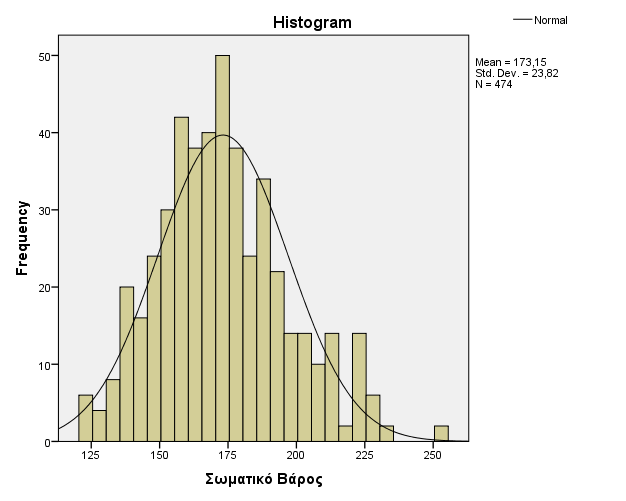
\includegraphics[width=0.7\textwidth]{images/16.png}
    \end{figure}
    
    Στη συνέχεια παρατίθενται τα θηκογράμματα των ποσοτικών μεταβλητών. Όπως παρατηρείται δεν υπάρχουν εξαιρετικά ακραίες τιμές (outliers – δηλαδή τιμές που ξεπερνάνε κατά 1,5 ή κατά 3 φορές το ενδοτεταρτημοριακό εύρος) μόνο για τη μεταβλητή  “Ηλικία πρώτου επεισοδίου”. 
    
    \clearpage
    \begin{figure}
 \centering
            \begin{subfigure}{0.7\textwidth}
     \centering
         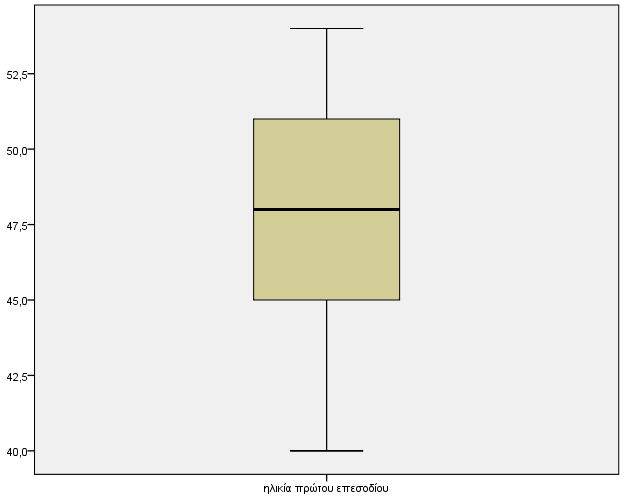
\includegraphics[width=\textwidth]{images/17.png}
                      \end{subfigure}
                      
     \begin{subfigure}{0.7\textwidth}
     \centering
      \vspace{1cm}
         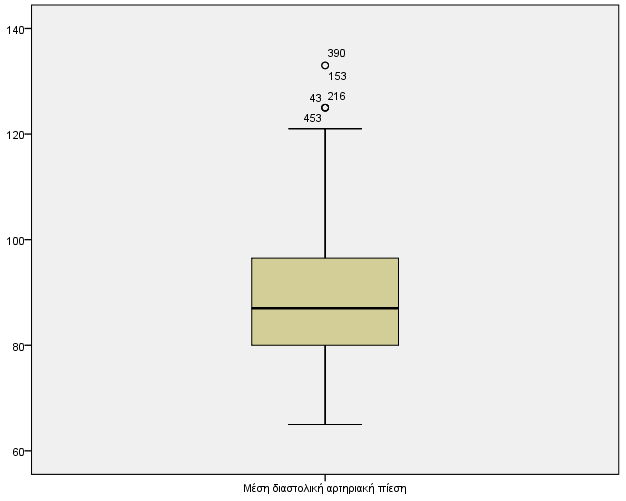
\includegraphics[width=\textwidth]{images/18.png}
                      \end{subfigure}
    \end{figure}
    
   \clearpage
    \begin{figure}
 \centering
            \begin{subfigure}{0.7\textwidth}
     \centering
         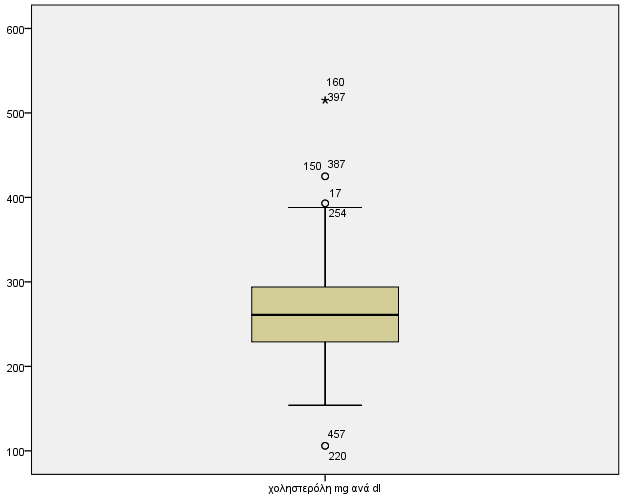
\includegraphics[width=\textwidth]{images/19.png}
                      \end{subfigure}
                      
     \begin{subfigure}{0.7\textwidth}
     \centering
     \vspace{1cm}
         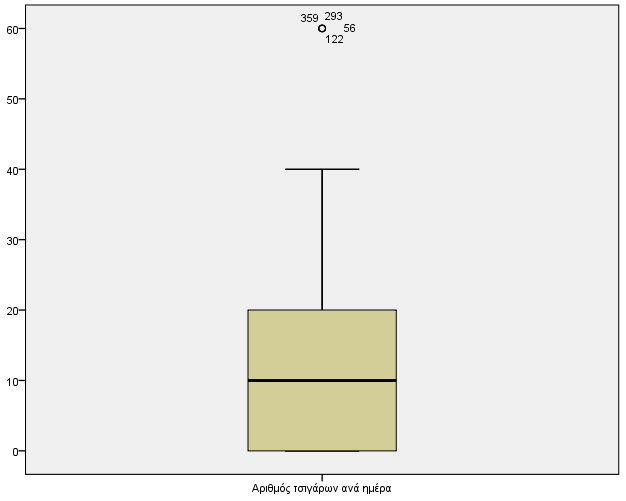
\includegraphics[width=\textwidth]{images/20.png}
                      \end{subfigure}
    \end{figure}
    
    \begin{figure}
        \centering
        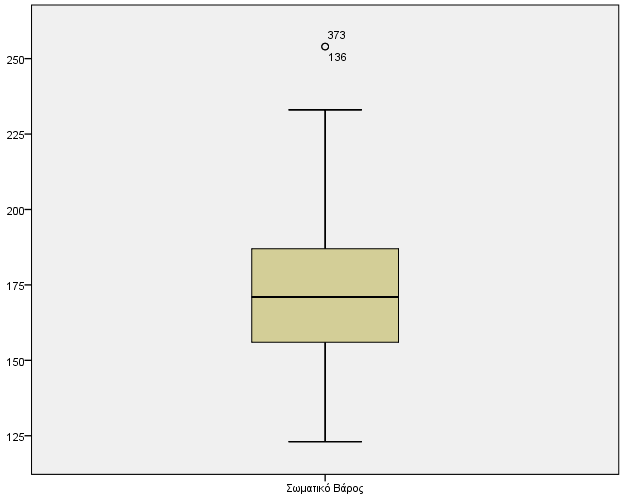
\includegraphics[width=0.7\textwidth]{images/21.png}
    \end{figure}
    
\clearpage
Στον ακόλουθο πίνακα παρουσιάζονται τα προεπιλεγμένα περιγραφικά στατιστικά στοιχεία για τη “Μέση διαστολική αρτηριακή πίεση” ανά κατηγορίες σοβαρότητας πρώτου καρδιακού επεισοδίου και οικογενειακού ιστορικού ΚΕ.
\begin{figure}[hb]
        \centering
        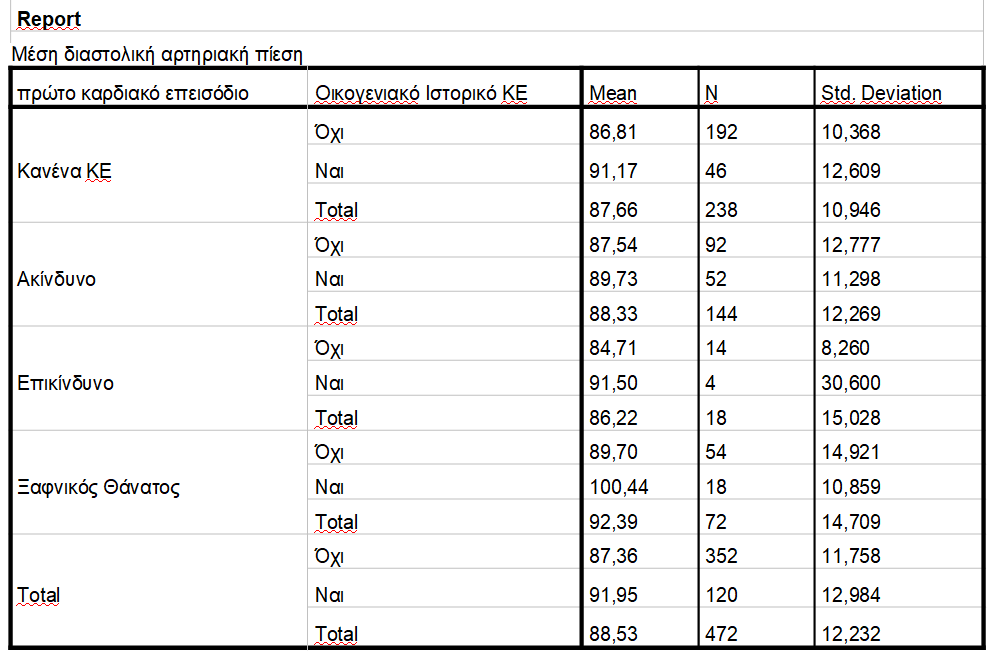
\includegraphics[width=0.7\textwidth]{images/22.PNG}
    \end{figure}
    
    Από τα στοιχεία του πίνακα παρατηρούμε πως τα άτομα τα οποία δεν έχουν οικογενειακό ιστορικό παρουσιάζουνε μικρότερες τιμές μέσης διαστολικής αρτηριακής πίεσης για όλες τις κατηγορίες της μεταβλητής “ πρώτο καρδιακό επεισόδιο “ . 
    
Επιπλέον φαίνεται να μην υπάρχει κάποια συστηματική αύξηση της μέσης διαστολικής αρτηριακής πίεσης για τις κατηγορίες του πρώτου καρδιακού επεισοδίου στο υπό μελέτη δείγμα. Το μόνο που μπορούμε να παρατηρήσουμε είναι πως τα άτομα της κατηγορίας ξαφνικός θάνατος έχουν την μεγαλύτερη τιμή μέσης διαστολικής αρτηριακής πίεσης (Total = 92,39). 

Τέλος,  παρατηρώντας τη στήλη που παρουσιάζει την τυπική απόκλιση της μέσης διαστολικής αρτηριακής πίεσης αξίζει να αναφερθεί ότι η μεγαλύτερη διασπορά γύρω από τη μέση διαστολική αρτηριακή πίεση εμφανίζεται στα άτομα με οικογενειακό ιστορικό στην κατηγορία επικίνδυνο ΚΕ (st.dev = 30,60).  

\clearpage
Στον ακόλουθο πίνακα παρουσιάζονται τα προεπιλεγμένα περιγραφικά στατιστικά στοιχεία για τη “Μέση διαστολική αρτηριακή πίεση” ανά κατηγορίες σοβαρότητας πρώτου καρδιακού επεισοδίου και επιβίωσης μετά από 10 χρόνια.

\begin{figure}[hb]
        \centering
        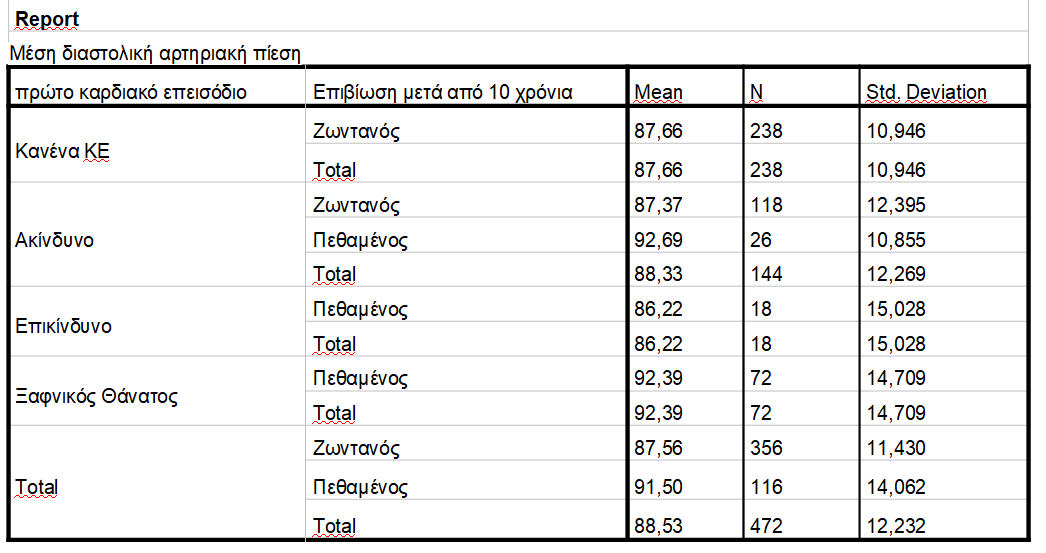
\includegraphics[width=0.7\textwidth]{images/23.PNG}
    \end{figure}
    
    Από τα στοιχεία του πίνακα παρατηρούμε πως στις κατηγορίες επικίνδυνο και ξαφνικός θάνατος της μεταβλητής πρώτο καρδιακό επεισόδιο δεν έχει επιβιώσει κανένας μετά από 10 χρόνια.
    
Επιπλέον φαίνεται να μην υπάρχει κάποια συστηματική αύξηση της μέσης διαστολικής αρτηριακής πίεσης για τις κατηγορίες του πρώτου καρδιακού επεισοδίου στο υπό μελέτη δείγμα. Το μόνο που μπορούμε να παρατηρήσουμε είναι πως τα άτομα της κατηγορίας ξαφνικός θάνατος έχουν την μεγαλύτερη τιμή μέσης διαστολικής αρτηριακής πίεσης (Total$=$92,39).  Στην επόμενη παράγραφο θα εξεταστεί αν οι διαφορές είναι στατιστικά σημαντικές.

Τέλος,  παρατηρώντας τη στήλη που παρουσιάζει την τυπική απόκλιση της μέσης διαστολικής αρτηριακής πίεσης αξίζει να αναφερθεί ότι η μεγαλύτερη διασπορά  εμφανίζεται στα άτομα τα οποία δεν έχουν επιβιώσει μετά από 10 χρόνια στην κατηγορία επικίνδυνο ΚΕ (st.dev = 15,028). 

\clearpage
Στον ακόλουθο πίνακα παρουσιάζονται τα προεπιλεγμένα περιγραφικά στατιστικά στοιχεία για τη “χοληστερόλη” ανά κατηγορίες σοβαρότητας πρώτου καρδιακού επεισοδίου και Οικογενειακό ιστορικό ΚΕ.

\begin{figure}[hb]
        \centering
        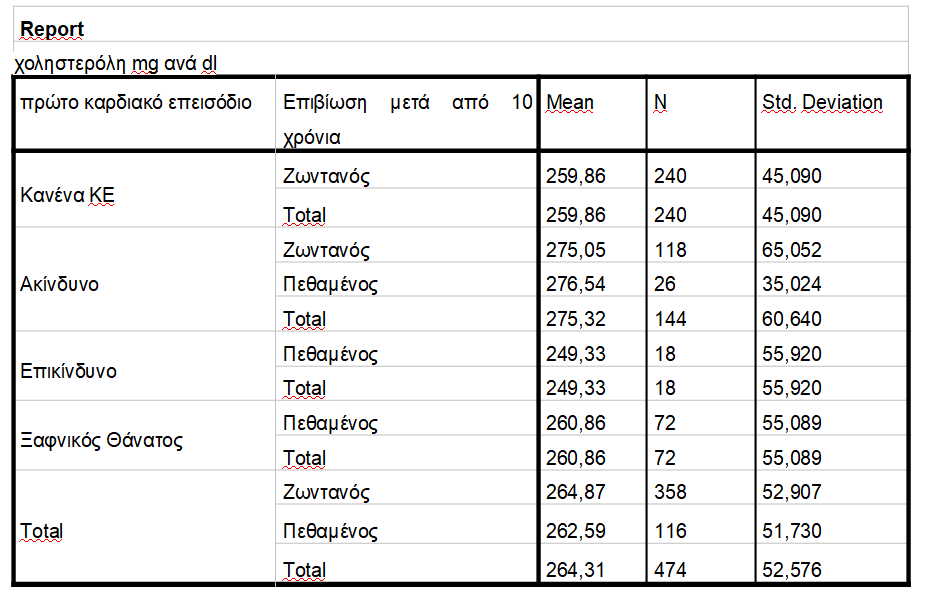
\includegraphics[width=0.7\textwidth]{images/24.PNG}
    \end{figure}
    
Από τα στοιχεία του πίνακα παρατηρούμε πως η μεγαλύτερη μέση τιμή για τη μεταβλητή χοληστερόλη παρατηρείται στα άτομα τα οποία δεν έχουν επιβιώσει μετά από 10 χρόνια για την κατηγορία ακίνδυνο της μεταβλητής πρώτο καρδιακό επεισόδιο (276,54) . 
Τέλος,  παρατηρώντας τη στήλη που παρουσιάζει την τυπική απόκλιση της χοληστερόλης αξίζει να αναφερθεί ότι η μεγαλύτερη διασπορά εμφανίζεται στα άτομα τα οποία έχουν επιβιώσει μετά από 10 χρόνια στην κατηγορία ακίνδυνο ΚΕ (st.dev = 65,052).

\clearpage
Στον ακόλουθο πίνακα παρουσιάζονται τα προεπιλεγμένα περιγραφικά στατιστικά στοιχεία για τη “Σωματικό Βάρος” ανά κατηγορίες σοβαρότητας πρώτου καρδιακού επεισοδίου και επιβίωσης μετά από 10 χρόνια.
\begin{figure}[hb]
        \centering
        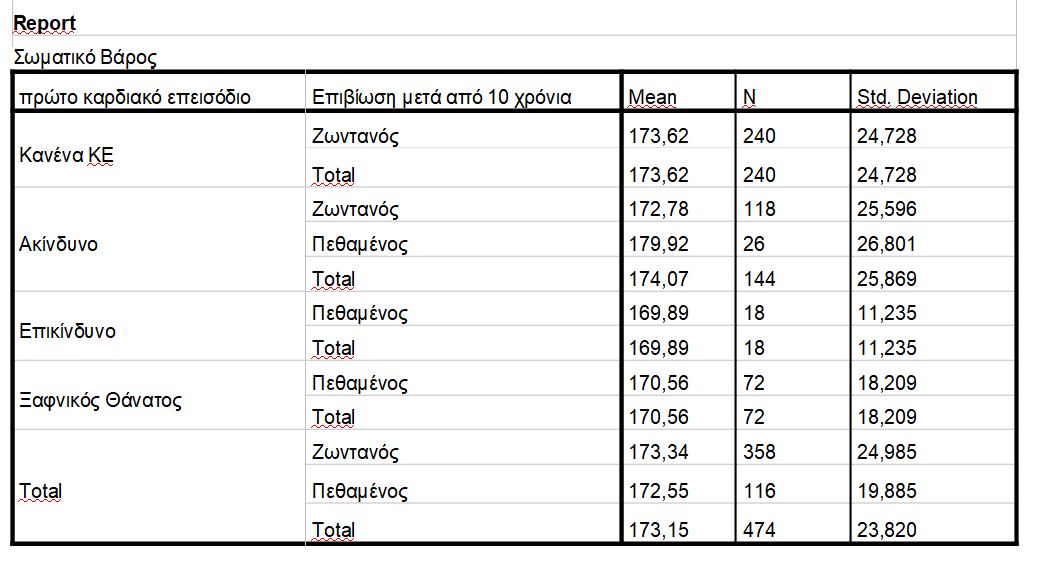
\includegraphics[width=0.7\textwidth]{images/25.PNG}
    \end{figure}
    
    Από τον πίνακα παρατηρούμε πως η μεγαλύτερη μέση τιμή για το Σωματικό Βάρος αναφέρεται στα άτομα τα οποία δεν έχουν επιβιώσει μετά από 10 χρόνια στην κατηγορία ακίνδυνο της μεταβλητής πρώτο καρδιακό επεισόδιο.
    
Επιπλέον φαίνεται να μην υπάρχει κάποια συστηματική αύξηση του Σωματικού Βάρους  για τις κατηγορίες του πρώτου καρδιακού επεισοδίου στο υπό μελέτη δείγμα. Το μόνο που μπορούμε να παρατηρήσουμε είναι πως τα άτομα της κατηγορίας ακίνδυνο έχουν την μεγαλύτερη τιμή Σωματικού Βάρους (Total = 174,07). 

Τέλος,  παρατηρώντας τη στήλη που παρουσιάζει την τυπική απόκλιση του Σωματικού Βάρους αξίζει να αναφερθεί ότι η μεγαλύτερη διασπορά εμφανίζεται στα άτομα τα οποία δεν έχουν επιβιώσει μετά από 10 χρόνια στην κατηγορία ακίνδυνο ΚΕ (st.dev = 26,801).

\clearpage
Στον ακόλουθο πίνακα παρουσιάζονται τα προεπιλεγμένα περιγραφικά στατιστικά στοιχεία για τον “Αριθμό τσιγάρων” ανά κατηγορίες σοβαρότητας πρώτου καρδιακού επεισοδίου και επιβίωσης μετά από 10 χρόνια.

\begin{figure}[hb]
        \centering
        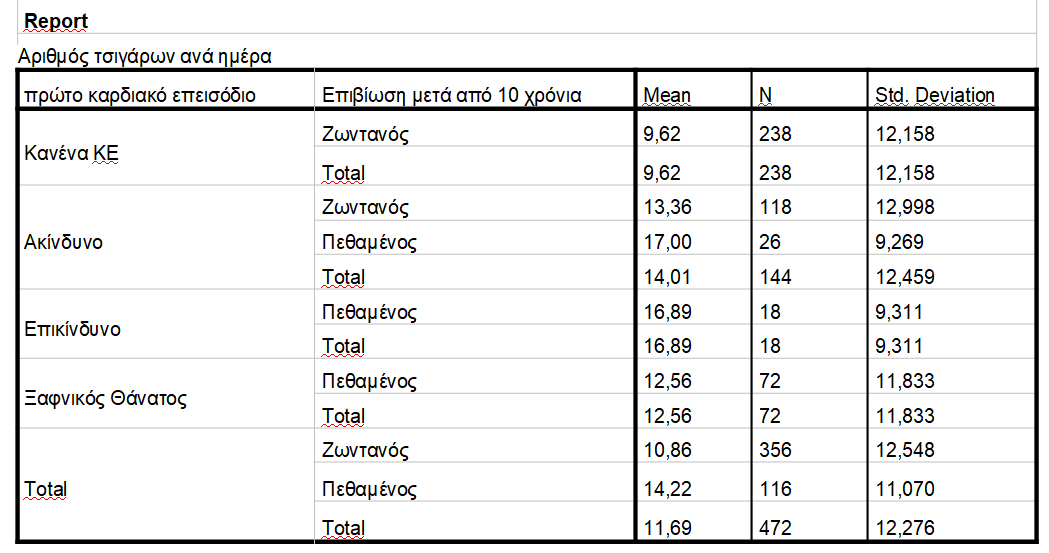
\includegraphics[width=0.7\textwidth]{images/26.PNG}
    \end{figure}
    
Από τον πίνακα φαίνεται να μην υπάρχει κάποια συστηματική αύξηση του Αριθμού τσιγάρων ανά ημέρα  για τις κατηγορίες του πρώτου καρδιακού επεισοδίου στο υπό μελέτη δείγμα. Παρ’ όλα αυτά φαίνεται να υπάρχουν στατιστικά σημαντικές διαφορές στις μέσες τιμές, κάτι το οποίο θα εξεταστεί στη συνέχεια της εργασίας. Το μόνο που μπορούμε να παρατηρήσουμε είναι πως τα άτομα της κατηγορίας επικίνδυνο πρώτο καρδιακό επεισόδιο έχουν την μεγαλύτερη τιμή Αριθμού τσιγάρων ανά ημέρα (Total = 16,89). 

Όσον αφορά τη σχέση της επιβίωσης μετά από 10 χρόνια με τον αριθμό των τσιγάρων ανά ημέρα, φαίνεται ότι όσοι δεν επιβίωσαν κάπνιζαν περισσότερο σε σχέση με αυτούς που επέζησαν. Η διαφορά αυτή στις μέσες τιμές θα εξεταστεί και παρακάτω. 

\clearpage
Ακολούθως, παρατίθενται τα συνδυαστικά διαγράμματα (clustered) μεταξύ των κατηγορικών μεταβλητών πρώτο καρδιακό επεισόδιο – επιβίωση μετά από 10 χρόνια – οικογενειακό ιστορικό ΚΕ.  
\begin{figure}[hb]
        \centering
        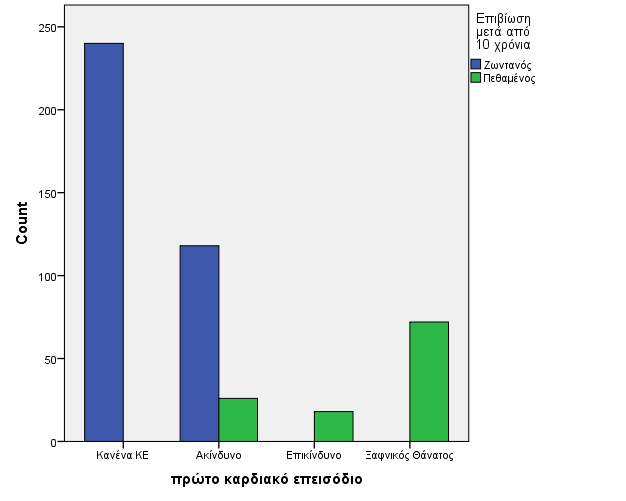
\includegraphics[width=0.8\textwidth]{images/27.png}
    \end{figure}
    
    Από το πρώτο συνδυαστικό διάγραμμα διαπιστώνουμε ότι το ποσοστό των ατόμων που έχουν επιβιώσει μετά από 10 χρόνια είναι πολύ μεγαλύτερο από αυτό των θανόντων για ακίνδυνο πρώτο καρδιακό επεισόδιο, ενώ στην υποκατηγορία επικίνδυνο δεν έχει επιβιώσει κανείς.  
    
    \clearpage
    \begin{figure}[hb]
        \centering
        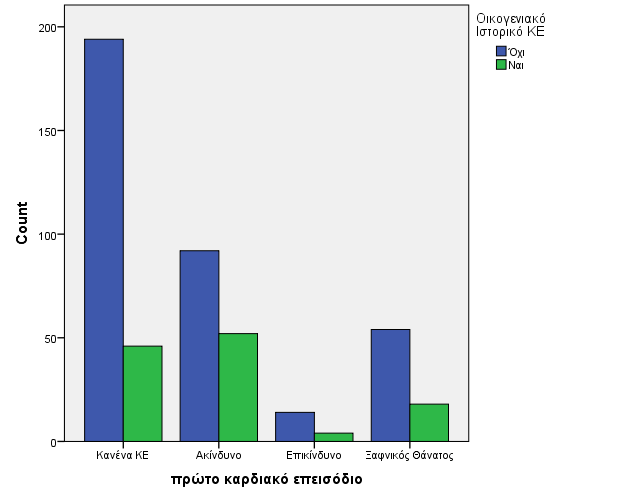
\includegraphics[width=0.8\textwidth]{images/28.png}
    \end{figure}
    Στο δεύτερο συνδυαστικό διάγραμμα αξίζει να τονιστεί ότι τα άτομα τα οποία δεν έχουν οικογενειακό ιστορικό και έχουν υποστεί ακίνδυνο, επικίνδυνο και ξαφνικό θάνατο λόγω πρώτου καρδιακού επεισοδίου είναι περισσότερα σε σχέση με αυτά που έχουν οικογενειακό ιστορικό.
    
    \clearpage
    \begin{figure}[hb]
        \centering
        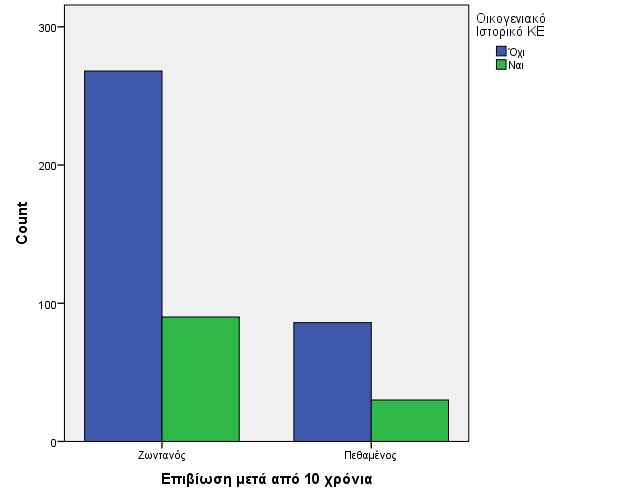
\includegraphics[width=0.8\textwidth]{images/29.png}
    \end{figure}
    
    Στο τρίτο συνδυαστικό διάγραμμα διαπιστώνεται ότι στα άτομα που δεν έχουν επιβιώσει μετά από 10 χρόνια μετά από καρδιακό επεισόδιο τα περισσότερα δεν είχαν οικογενειακό ιστορικό ΚΕ.  
\clearpage
\section{Έλεγχοι με επαγωγικές διαδικασίες και η στατιστική ερμηνεία τους (Β \& Γ)}

\subsection{Έλεγχος ανεξαρτησίας \lat{$X^2$}}
Με βάση τα παραπάνω στοιχεία τα οποία  είναι αποτέλεσμα του ερωτήματος Α απορρέουν μερικά ερωτήματα τα οποία μπορούν να ελεγχθούν με συγκεκριμένες επαγωγικές διαδικασίες.

Αρχικά, θα ήταν σκόπιμο να ελέγξουμε την ανεξαρτησία ορισμένων μεταβλητών οι οποίες θεωρούνται χαρακτηριστικές. \textbf{Η σχέση ανάμεσα στην μεταβλητή "Πρώτο καρδιακό επεισόδιο" και την "Οικογενειακό ιστορικό" θα ήταν ενδιαφέρον να ερευνηθεί για τυχόν ύπαρξη σχέσης ανάμεσα τους.}

Με την εφαρμογή του ελέγχου ανεξαρτησίας \lat{$X^2$} παίρνουμε τις παρακάτω πληροφορίες σε μορφή πινάκων.

\begin{figure}[h]
    \centering
    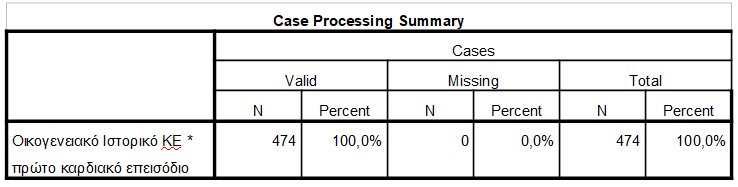
\includegraphics[width=0.8\textwidth]{images/100.PNG}
\end{figure}

Στον πίνακα \textbf{Case Processing Summary},όπως και παραπάνω με τον πίνακα \textbf{Statistics} μπορούμε να πάρουμε πληροφορίες για τυχόν cases που δεν συμπεριλήφθησαν από την στήλη Missing. Όπως είναι εμφανές, από ένα σύνολο 474 cases, όλες λήφθησαν υπόψη.

\begin{figure}[h]
    \centering
    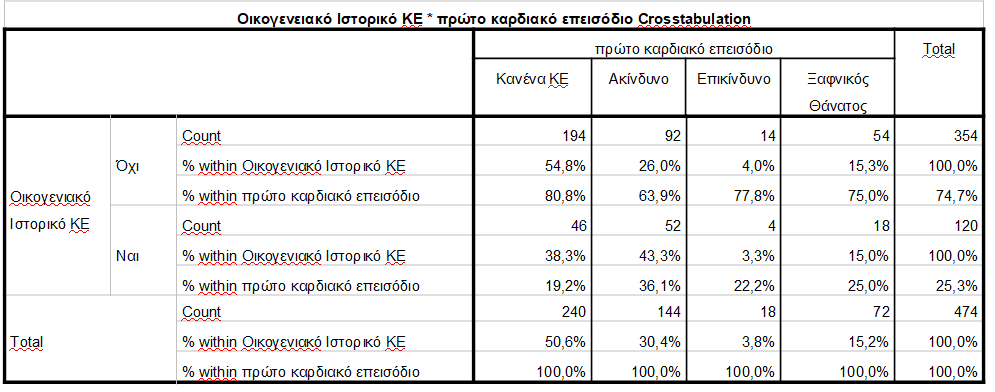
\includegraphics[width=\textwidth]{images/101.PNG}
\end{figure}

Από τον πίνακα συνάφειας παρατηρούμε τα εξής: 
\begin{itemize}
    \item Όσοι δεν είχαν κανένα καρδιακό επεισόδιο χωρίς οικογενειακό ιστορικό (80,8\%) εμφανίζουν μεγαλύτερο ποσοστό σε σχέση με όσους είχαν οικογενειακό ιστορικό (19,2\%).
    \item Όσοι υπέστησαν ακίνδυνο καρδιακό επεισόδιο χωρίς οικογενειακό ιστορικό (63,9\%) είναι σχεδόν διπλάσιοι σε ποσοστό σε σχέση με αυτούς που είχαν οικογενειακό ιστορικό (36,1\%). 
    \item Επιπλέον παρατηρείται ότι το ποσοστό εμφάνισης καρδιακού επεισοδίου (από κανένα σε ακίνδυνο καρδιακό) αυξάνεται σχεδόν στο διπλάσιο για όσους έχουν οικογενειακό ιστορικό.
\end{itemize}

\begin{figure}[h]
    \centering
    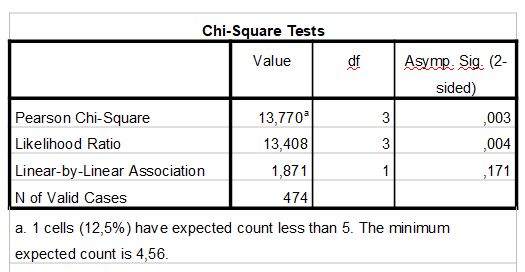
\includegraphics[width=0.8\textwidth]{images/102.PNG}
\end{figure}

Στον πίνακα \lat{Chi-Square Tests} παρατηρούμε ότι \lat{$X^2=13,77$} και p=0,003. Δηλαδή, πρόκειται για ένα στατιστικά σημαντικό τεστ. Επιπλέον, δεδομένου ότι το \lat{$p<0,05$},  μπορούμε να συμπεράνουμε ότι οι μεταβλητές  "Οικογενειακό Ιστορικό" και "Πρώτο Καρδιακό Επεισόδιο" συσχετίζονται η μία με την άλλη. Κατά συνέπεια, απορρίπτουμε την μηδενική υπόθεση καθώς \textbf{υπάρχει εξάρτηση ανάμεσα στις δύο αυτές μεταβλητές}.

Στην συνέχεια θα μελετήσουμε την σχέση εξάρτησης ανάμεσα στις μεταβλητές "Πρώτο Καρδιακό Επεισόδιο" και "Επιβίωση μετά από 10 χρόνια". 

\begin{figure}[h]
    \centering
    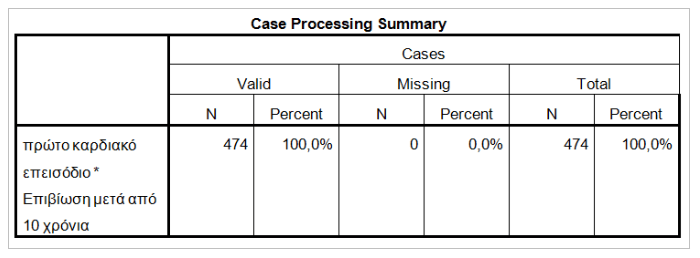
\includegraphics[width=0.8\textwidth]{images/103.PNG}
\end{figure}

Στον πίνακα \textbf{Case Processing Summary}, όπως και προηγουμένως παρατηρούμε ότι όλες οι τιμές λήφθησαν υπόψιν.
\clearpage

\begin{figure}[h]
    \centering
    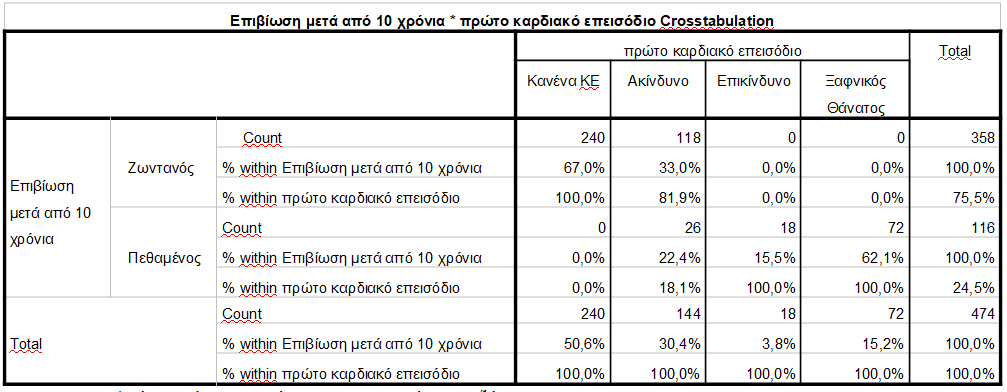
\includegraphics[width=\textwidth]{images/104.PNG}
\end{figure}

Από τον πίνακα συνάφειας παρατηρούμε τα εξής:
\begin{itemize}
    \item Για όσους δεν υπέστησαν κανένα καρδιακό επεισόδιο η θνησιμότητα είναι μηδενική μετά από 10 χρόνια. 
    \item Σε όσους υπέστησαν ακίνδυνο πρώτο καρδιακό επεισόδιο το μεγαλύτερο ποσοστό παρέμεινε ζωντανό μετά από 10 χρόνια (81,9\%) σε σχέση με όσους απεβίωσαν (18,1\%).
    \item Όσον αφορά τις υποκατηγορίες επικίνδυνο και ξαφνικός θάνατος τα αποτελέσματα που προέκυψαν είναι απολύτως λογικά, καθώς η θνησιμότητα φτάνει σε ποσοστό 100\%.
\end{itemize}

\begin{figure}[h]
    \centering
    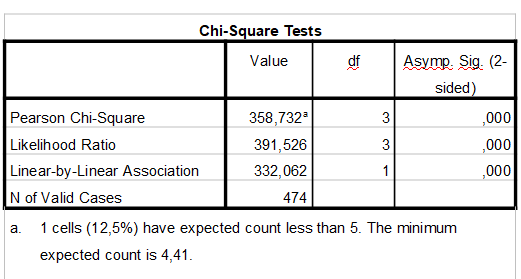
\includegraphics[width=0.8\textwidth]{images/105.PNG}
\end{figure}

Στον πίνακα Chi-Square Tests παρατηρούμε ότι \lat{$X^2=358,73$} και p=0,0001. Δηλαδή, πρόκειται για ένα στατιστικά σημαντικό τεστ. Επιπλέον, δεδομένου ότι το \lat{$p<0,05$}, μπορούμε να συμπεράνουμε ότι οι μεταβλητές  "Πρώτο Καρδιακό Επεισόδιο" και "Επιβίωση μετά από 10 χρόνια" συσχετίζονται η μία με την άλλη. Κατά συνέπεια, απορρίπτουμε την μηδενική υπόθεση καθώς \textbf{υπάρχει εξάρτηση ανάμεσα στις δύο αυτές μεταβλητές}.

\clearpage
Στην συνέχεια θα μελετήσουμε την σχέση εξάρτησης ανάμεσα στις μεταβλητές "Οικογενειακό Ιστορικό ΚΕ" και "Επιβίωση μετά από 10 χρόνια".

\begin{figure}[h]
    \centering
    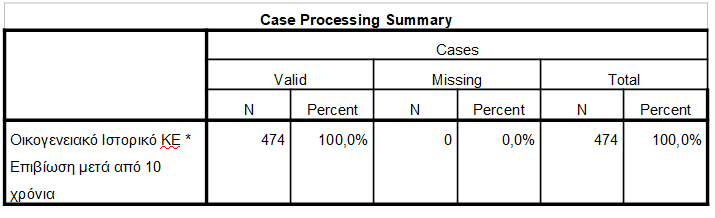
\includegraphics[width=0.8\textwidth]{images/106.PNG}
\end{figure}

Στον πίνακα \textbf{Case Processing Summary},όπως και προηγουμένως παρατηρούμε ότι όλες οι τιμές λήφθησαν υπόψη. 

\begin{figure}[h]
    \centering
    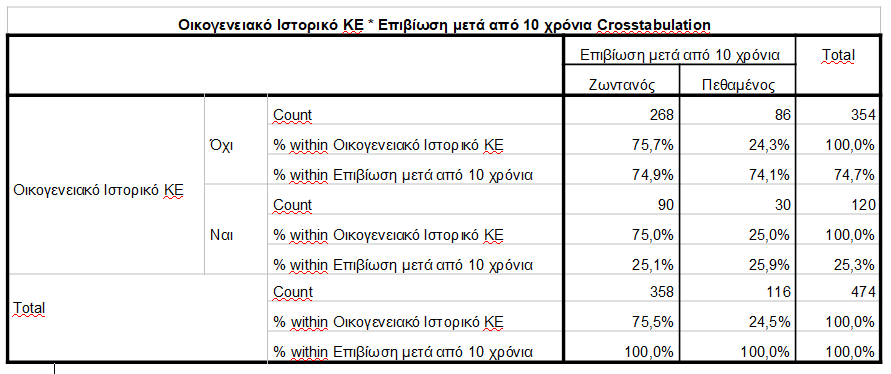
\includegraphics[width=\textwidth]{images/107.PNG}
\end{figure}

Από τον πίνακα συνάφειας παρατηρούμε τα εξής:
\begin{itemize}
    \item Το ποσοστό των ατόμων που επιβίωσαν μετά από 10 χρόνια χωρίς να έχουν οικογενειακό ιστορικό ΚΕ είναι περισσότεροι σε σχέση με αυτούς που έχουν.
    \item Αυτό που αξίζει να τονιστεί είναι πως το ποσοστό των ατόμων που απεβίωσαν μετά από 10 χρόνια είναι μεγαλύτερο για όσους δεν έχουν οικογενειακό ιστορικό ΚΕ (74,1\%) σε σχέση με όσους έχουν (25,9\%).
\end{itemize}

\clearpage

\begin{figure}[h]
    \centering
    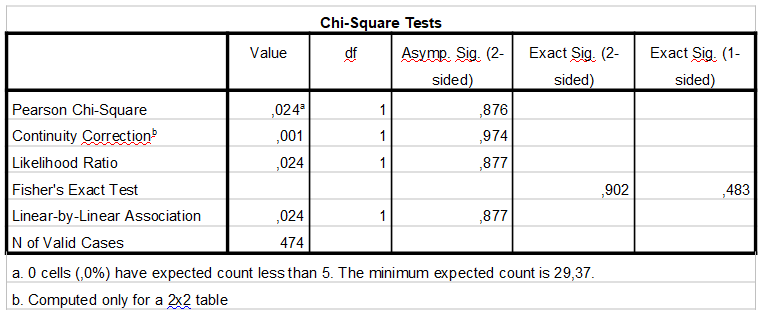
\includegraphics[width=0.8\textwidth]{images/108.PNG}
\end{figure}

Στον πίνακα \lat{Chi-Square Tests} παρατηρούμε ότι \lat{$X^2=0,024$} και p=0,876. Είναι προφανές ότι δεν υπάρχει ιδιαίτερη συσχέτιση ανάμεσα στις δύο μεταβλητές. Συγκεκριμένα, από την τιμή του p-value η οποία είναι μεγαλύτερη του 5\% μπορούμε να πούμε ότι οι δύο αυτές μεταβλητές \textbf{είναι ανεξάρτητες μεταξύ τους}.

Αξίζει να σημειωθεί πως το ποσοστό που υπάρχει στην παρένθεση της υποσημείωσης σε όλους τους πίνακες \lat{$\textbf{X}^\textbf{2}$} αναφέρεται στο ποσοστό των αναμενόμενων συχνοτήτων που είναι μικρότερες από 5 και δεν ξεπερνάει το 20\%.

\subsection{Έλεγχοι διαφορών ως προς μεταβλητές \lat{nominal}}

\subsubsection{Έλεγχος κανονικότητας}

Ξεκινώντας με τις μεταβλητές "Αριθμός Τσιγάρων ανά Ημέρα" και "Επιβίωση μετά από 10 χρόνια". Μέσω του ελέγχου ως προς την κανονική κατανομή με το \lat{Kolmogorov-Smirnov} και \lat{Shapiro-Wilk} παίρνουμε τους παρακάτω πίνακες και διαγράμματα. 

\begin{figure}[h]
    \centering
    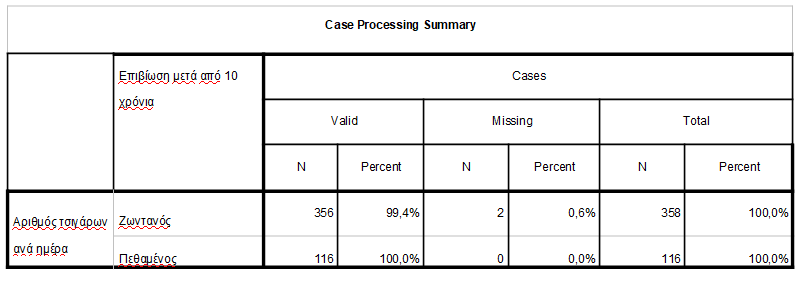
\includegraphics[width=0.8\textwidth]{images/109.PNG}
\end{figure}

Ο πίνακας \textbf{Case Processing Summary}, όπως και προηγουμένως μας δίνει πληροφορίες για το πόσα από τα cases που υπήρχαν αρχικά στο αρχείο μας, λήφθηκαν υπόψιν.

\clearpage

\begin{figure}[h]
    \centering
    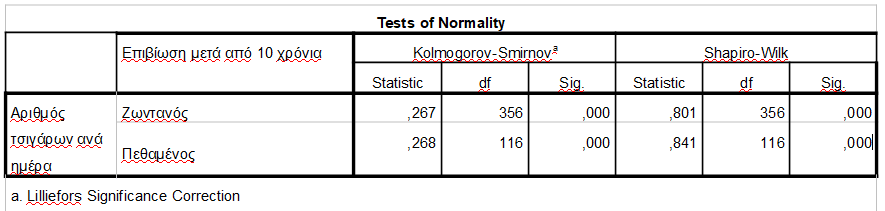
\includegraphics[width=0.8\textwidth]{images/110.PNG}
\end{figure}

Από τον πίνακα \lat{Tests of Normality} μπορούμε να πάρουμε αποτελέσματα από δύο τεστ κανονικότητας, τα \lat{Kolmogorov-Smirnov} και \lat{Shapiro-Wilk}.Το δεύτερο χρησιμοποιείται κυρίως για μικρά δείγματα ενώ το πρώτο δίνει καλά  αποτελέσματα και για μεγάλα. Στην περίπτωση μας έχουμε δείγμα από 474 ασθενείς οπότε θα χρησιμοποιήσουμε το πρώτο. Παρατηρώντας τον πίνακα βλέπουμε ότι το p-value και στις δύο περιπτώσεις είναι κατά πολύ μικρότερο του 5\%. Συνεπώς, τα δεδομένα μας αποκλίνουν από την κανονικότητα.

Αποτελέσματα για την κανονικότητα μπορούμε να πάρουμε και γραφικά μέσω των \lat{Q-Q plots}. Όπως βλέπουμε και στα δύο διαγράμματα, τα δεδομένα μας έχουν την τάση να απομακρυνθούν από την διαγώνιο. Κατά συνέπεια, τα διαγράμματα όπως ήταν αναμενόμενο συμφωνούν με τον πίνακα.


\begin{figure}[h]
    \centering
    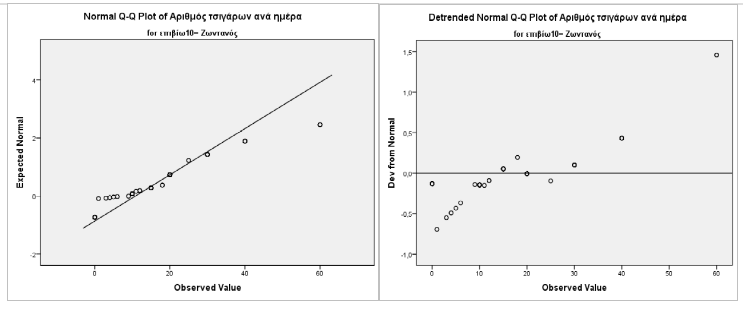
\includegraphics[width=0.8\textwidth]{images/111.PNG}
\end{figure}

\begin{figure}[h]
    \centering
    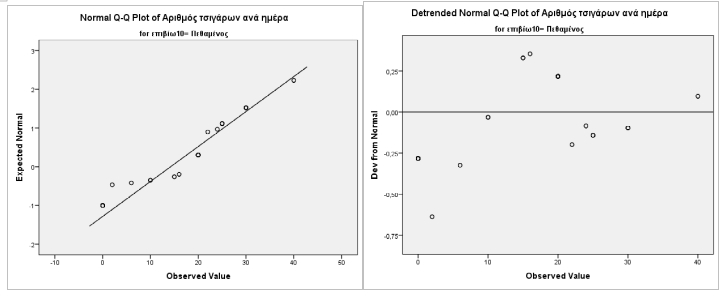
\includegraphics[width=0.8\textwidth]{images/112.PNG}
\end{figure}

\clearpage

\begin{figure}[h]
    \centering
    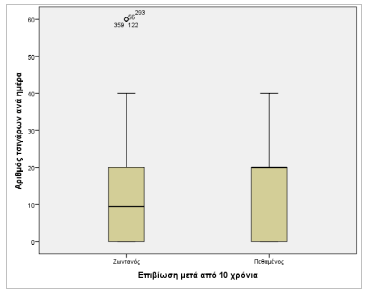
\includegraphics[width=0.8\textwidth]{images/113.PNG}
\end{figure}

Παρατηρούμε ότι από τον πίνακα \textbf{\lat{Test Statistics}} υπάρχει σημαντική διαφορά ανάμεσα στις μέσες τιμές των μεταβλητών Επιβίωση μετά από 10 χρόνια και Αριθμού τσιγάρων σύμφωνα με το \lat{Mann-Whitney}. Αυτό προκύπτει από το γεγονός ότι το p-value είναι <5\%. Συμπεραίνουμε  ότι τα άτομα που δεν επιβίωσαν είχαν την τάση να καπνίζουν περισσότερα τσιγάρα.

\vspace{2cm}

 \begin{figure}[h]
     \centering
     \begin{subfigure}{0.8\textwidth}
     \centering
         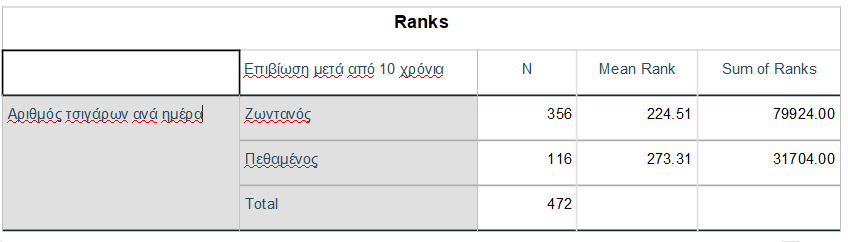
\includegraphics[width=\textwidth]{images/114.PNG}
              \end{subfigure}
              \end{figure}
     
     \clearpage
     
     \begin{figure}[ht]\ContinuedFloat
     \centering
     \begin{subfigure}{0.8\textwidth}
     \centering
         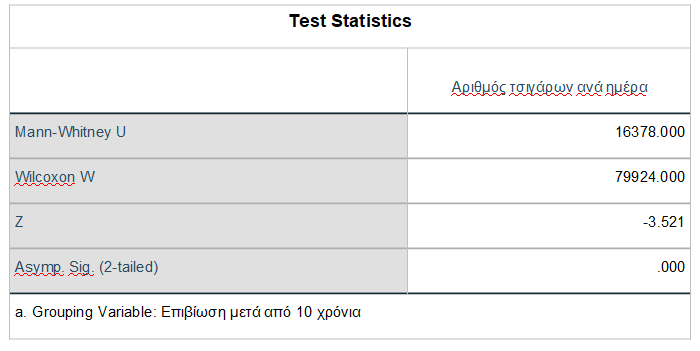
\includegraphics[width=\textwidth]{images/115.PNG}
             \end{subfigure}
      
\end{figure}

Ο πίνακας \textbf{\lat{Case Processing Summary}}  μας δίνει πληροφορίες για το πόσα από τα cases που υπήρχαν αρχικά στο αρχείο μας, λήφθηκαν υπόψιν.

\begin{figure}[h]
    \centering
    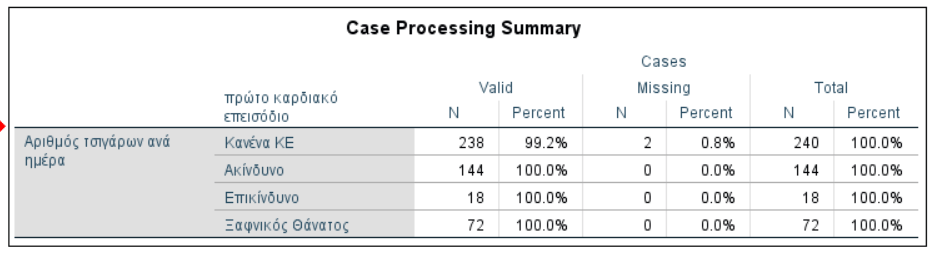
\includegraphics[width=\textwidth]{images/200.PNG}
\end{figure}

\vspace{1cm}
Από τον πίνακα Tests of Normality μπορούμε να πάρουμε αποτελέσματα από δύο τεστ κανονικότητας, τα Kolmogorov-Smirnov και Shapiro-Wilk. Παρατηρώντας τον πίνακα βλέπουμε ότι το p-value και στις δύο περιπτώσεις είναι κατά πολύ μικρότερο του 5\%.  Άρα οι μεταβλητές μας δεν ακολουθούν κανονική κατανομή.

Όσο αναφορά την κατηγορία “Επικίνδυνο” έχουμε λίγες μετρήσεις και αρκετές ακραίες τιμές. Όμως η αφαίρεση τους αφήνει το δείγμα με 12 μόνο μετρήσεις με αποτέλεσμα τα \lat{tests} κανονικότητας να μην δίνουν αποτελέσματα. Αξίζει να αναφέρουμε ότι τα δεδομένα για αυτήν την κατηγορία προφανώς δεν είναι αρκετά αλλά από ερευνητική σκοπιά κρίναμε αναγκαίο να μελετηθούν οι επιπτώσεις του τσιγάρου όσο αναφορά το “πρώτο καρδιακό επεισόδιο”. Επιπλέον οι μη παραμετρικοί έλεγχοι  μπορούν να εφαρμοστούν σε περιπτώσεις πολύ μικρών δειγμάτων.

\clearpage

\begin{figure}[h]
    \centering
    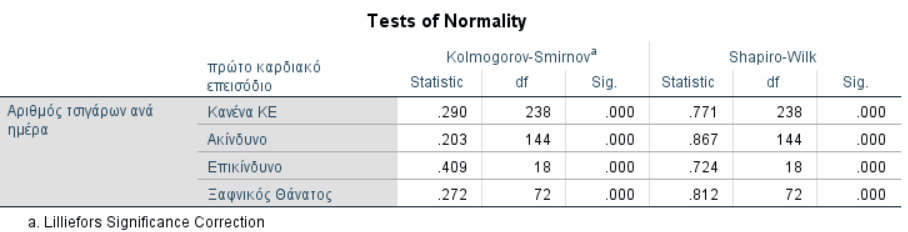
\includegraphics[width=\textwidth]{images/201.PNG}
\end{figure}

\vspace{1cm}

\begin{figure}[h]
 \centering

     \begin{subfigure}{0.8\textwidth}
     \centering
         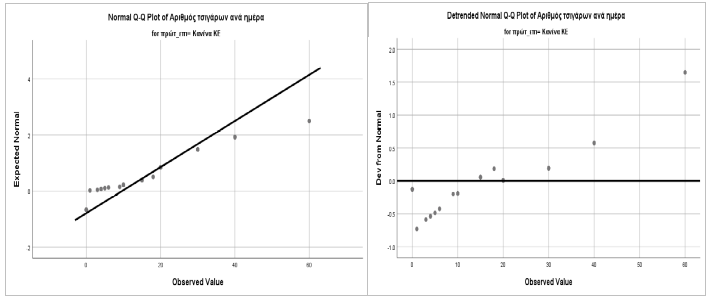
\includegraphics[width=\textwidth]{images/300.PNG}
                      \end{subfigure}
     \vspace{1cm}
     
     \begin{subfigure}{0.8\textwidth}
     \centering
         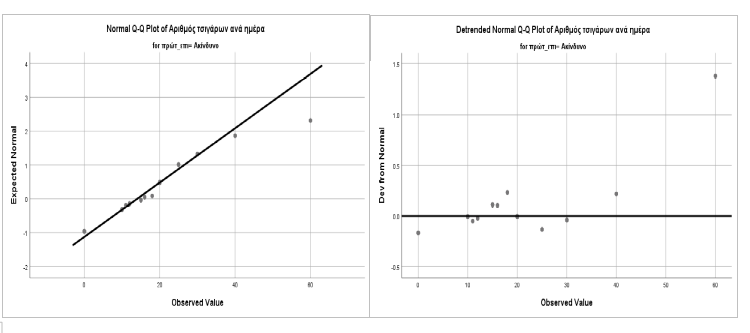
\includegraphics[width=\textwidth]{images/301.PNG}
             \end{subfigure}
\end{figure}

\clearpage

\begin{figure}
 \centering

     \begin{subfigure}{0.8\textwidth}
     \centering
         \includegraphics[width=\textwidth]{images/302.PNG}
                      \end{subfigure}
                      
     \vspace{2cm}
     
     \begin{subfigure}{0.8\textwidth}
     \centering
         \includegraphics[width=\textwidth]{images/303.PNG}
             \end{subfigure}
\end{figure}

\clearpage

\begin{figure}[ht]
    \centering
    \includegraphics[width=\textwidth]{images/304.png}
\end{figure}

Παρατηρούμε ότι από τον πίνακα \textbf{\lat{Test Statistics}} υπάρχει σημαντική διαφορά ανάμεσα στις μέσες τιμές των μεταβλητών "Πρώτο καρδιακό επεισόδιο" και τον "Αριθμό τσιγάρων". Αυτό προκύπτει από το γεγονός ότι το p-value είναι <5\%.  Συμπεραίνουμε ότι ο αριθμός τσιγάρων φαίνεται να επηρεάζει την επικινδυνότητα του πρώτου καρδιακού επεισοδίου.

\begin{figure}[h]
    \centering
    \includegraphics[width=0.9\textwidth]{images/202.PNG}
\end{figure}

\clearpage

\begin{figure}[ht]
    \centering
    \includegraphics[width=0.4\textwidth]{images/203.PNG}
\end{figure}

Εφόσον το \lat{Kruskal-Wallis} δείχνει ότι υπάρχουν σημαντικές διαφορές στις μέσες τιμές, θα πραγματοποιήσουμε τον έλεγχο \lat{Mann-Whitney}, ώστε να εντοπιστούν οι κατηγορίες στις οποίες εμφανίζονται οι διαφορές. 

\vspace{1cm}

\begin{figure}[ht]
    \centering
    \includegraphics[width=0.8\textwidth]{images/204.PNG}
\end{figure}

\vspace{1cm}
Παρατηρούμε ότι από τον πίνακα \textbf{\lat{Test Statistics}} υπάρχει σημαντική διαφορά ανάμεσα στις μέσες τιμές των μεταβλητών "Κανένα ΚΕ" και "Ακίνδυνο" σε σχέση με τον "Αριθμό τσιγάρων". Αυτό προκύπτει από το γεγονός ότι το p-value είναι <5\%. Συμπεραίνουμε  ότι τα άτομα που είναι στην κατηγορία "Κανένα ΚΕ"  είχαν την τάση να καπνίζουν λιγότερα τσιγάρα σε σχέση με αυτά της κατηγορίας "Ακίνδυνο".

\clearpage

\begin{figure}[ht]
    \centering
    \includegraphics[width=0.4\textwidth]{images/205.PNG}
\end{figure}

Για τις διαφορές “Κανένα ΚΕ” και “Επικίνδυνο” φαίνεται και εδώ στατιστικά σημαντική διαφορά στις μέσες τιμές σε σχέση με τον “Αριθμό τσιγάρων”. Αυτό προκύπτει από το γεγονός ότι το p-value είναι <5\%. Φαίνεται να καπνίζουν λιγότερο τα άτομα στην κατηγορία “Κανένα ΚΕ” σε σχέση με αυτούς στην κατηγορία “Επικίνδυνο”.

\vspace{1cm}

\begin{figure}[h]
    \centering
    \includegraphics[width=0.8\textwidth]{images/206.PNG}
\end{figure}

\vspace{1cm}

\begin{figure}[h]
    \centering
    \includegraphics[width=0.4\textwidth]{images/207.PNG}
\end{figure}

\clearpage

Για τις διαφορές “Κανένα ΚΕ” και “Ξαφνικός θάνατος” φαίνεται και εδώ στατιστικά σημαντική διαφορά στις μέσες τιμές σε σχέση με τον “Αριθμό τσιγάρων”. Αυτό προκύπτει από το γεγονός ότι το p-value είναι <5\%. Φαίνεται να καπνίζουν λιγότερο τα άτομα στην κατηγορία “Κανένα ΚΕ” σε σχέση με αυτούς στην κατηγορία “Ξαφνικός θάνατος”.

\vspace{1cm}

\begin{figure}[h]
    \centering
    \includegraphics[width=0.8\textwidth]{images/208.PNG}
\end{figure}

\vspace{1cm}

\begin{figure}[h]
    \centering
    \includegraphics[width=0.4\textwidth]{images/209.PNG}
\end{figure}

Για τις διαφορές “Ακίνδυνο” και “Επικίνδυνο” φαίνεται ότι δεν υπάρχει στατιστικά σημαντική διαφορά στις μέσες τιμές σε σχέση με τον “Αριθμό τσιγάρων”. Αυτό προκύπτει από το γεγονός ότι το p-value είναι >5\%. Δηλαδή ο αριθμός τσιγάρων που καπνίζεται από τις δυο κατηγορίες είναι ίδιος.

\begin{figure}[h]
    \centering
    \includegraphics[width=0.8\textwidth]{images/210.PNG}
\end{figure}

\clearpage

\begin{figure}[ht]
    \centering
    \includegraphics[width=0.4\textwidth]{images/211.PNG}
\end{figure}

Για τις διαφορές “Ακίνδυνο” και “Ξαφνικός θάνατος” φαίνεται ότι δεν υπάρχει στατιστικά σημαντική διαφορά στις μέσες τιμές σε σχέση με τον “Αριθμό τσιγάρων”. Αυτό προκύπτει από το γεγονός ότι το p-value είναι >5\%. Δηλαδή ο αριθμός τσιγάρων που καπνίζεται από τις δυο κατηγορίες είναι ίδιος.

\vspace{1cm}

\begin{figure}[h]
    \centering
    \includegraphics[width=0.8\textwidth]{images/212.PNG}
\end{figure}
\vspace{1cm}
\begin{figure}[h]
    \centering
    \includegraphics[width=0.4\textwidth]{images/213.PNG}
\end{figure}

\clearpage

\vspace{2cm}
Για τις διαφορές “Επικίνδυνο” και “Ξαφνικός θάνατος” φαίνεται ότι δεν υπάρχει στατιστικά σημαντική διαφορά στις μέσες τιμές σε σχέση με τον “Αριθμό τσιγάρων”. Αυτό προκύπτει από το γεγονός ότι το p-value είναι >5\%. Δηλαδή ο αριθμός τσιγάρων που καπνίζεται από τις δυο κατηγορίες είναι ίδιος.

\vspace{1cm}

\begin{figure}[h]
    \centering
    \includegraphics[width=0.8\textwidth]{images/214.PNG}
\end{figure}
\vspace{1cm}
\begin{figure}[h]
    \centering
    \includegraphics[width=0.4\textwidth]{images/215.PNG}
\end{figure}

\clearpage
Ο πίνακας \lat{Case Processing Summary}  μας δίνει πληροφορίες για το πόσα από τα \lat{cases} που υπήρχαν αρχικά στο αρχείο μας, λήφθηκαν υπόψιν, στην μελέτη των κατηγοριών του "Πρώτου καρδιακού επισοδείου" σε σχέση με την "Μέση διαστολική αρτηριακή πίεση".

\begin{figure}[h]
    \centering
    \includegraphics[width=\textwidth]{images/125.PNG}
\end{figure}
\vspace{1cm}
Από τον πίνακα \textbf{\lat{Tests of Normality}} μπορούμε να πάρουμε αποτελέσματα από δύο τεστ κανονικότητας, τα \lat{Kolmogorov-Smirnov} και \lat{Shapiro-Wilk}. Παρατηρώντας τον πίνακα βλέπουμε ότι το p-value εκτός της υποομάδας που έχει τον χαρακτηρισμό Επικίνδυνο, είναι μικρότερο του 5\%. Δηλαδή, δεν ακολουθούν κανονική κατανομή.  Λόγω αυτού, θα  χρησιμοποιήσουμε τον μη-παραμετρικό έλεγχο διαφορών ανάμεσα σε περισσότερες από δύο ανεξάρτητες ομάδες, \lat{Kruskal-Wallis H}. 
\vspace{1cm}
\begin{figure}[h]
    \centering
    \includegraphics[width=\textwidth]{images/126.PNG}
\end{figure}

\clearpage

\begin{figure}[h]
 \centering

     \begin{subfigure}{0.8\textwidth}
     \centering
         \includegraphics[width=\textwidth]{images/127.PNG}
                      \end{subfigure}
     
     \begin{subfigure}{0.8\textwidth}
     \centering
         \includegraphics[width=\textwidth]{images/128.PNG}
                    \end{subfigure}
                    
                    \begin{subfigure}{0.8\textwidth}
     \centering
         \includegraphics[width=\textwidth]{images/129.PNG}
                    \end{subfigure}
                    
                    \begin{subfigure}{0.8\textwidth}
     \centering
         \includegraphics[width=\textwidth]{images/130.PNG}
                    \end{subfigure}
\end{figure}

\clearpage

\begin{figure}[ht]
    \centering
    \includegraphics[width=\textwidth]{images/131.PNG}
\end{figure}

Από τον πίνακα \textbf{\lat{Test Statistics}} προκύπτει ότι  το p-value είναι >5\%. Συνεπώς δεν υπάρχουν σημαντικές διαφορές στη τιμή της  Μέσης διαστολικής αρτηριακής πίεσης σε σχέση με το πρώτο καρδιακό επεισόδιο. Άρα, η μέση διαστολική αρτηριακή πίεση φαίνεται να μην επηρεάζεται παρόλο την κατηγορία επικινδυνότητας του πρώτου καρδιακού επεισοδίου.

\begin{figure}[h]
    \centering
    \includegraphics[width=0.8\textwidth]{images/132.PNG}
\end{figure}

\clearpage

\begin{figure}[ht]
    \centering
    \includegraphics[width=0.6\textwidth]{images/133.PNG}
\end{figure}
\clearpage
\section{Λογαριθμική Παλινδρόμηση (Δ)}

Η λογαριθμική παλινδρόμηση χρησιμοποιείται για την εκτίμηση της πιθανότητας p της επιτυχίας μιας δίτιμης μεταβλητής για ένα σύνολο τιμών μίας ή περισσότερων ανεξάρτητων μεταβλητών. 
Για τη δημιουργία του λογαριθμικού μας μοντέλου χρησιμοποιήσαμε ως εξαρτημένη μεταβλητή την Επιβίωση μετά από 10 χρόνια και ως ανεξάρτητες το Πρώτο καρδιακό επεισόδιο , την Ηλικία και τη Μέση διαστολική αρτηριακή πίεση. 

Σημειώνεται πως έγινε επανακωδικοποίηση της μεταβλητής Πρώτο καρδιακό επεισόδιο ως εξής:



\begin{center}
 \begin{tabular}{|l|l|} 
 \hline
\hspace{1.2cm} \textbf{Αρχικά} & \hspace{1.2cm} \textbf{Τελικά} \\ [0.5ex]
 \hline
 1 $=$ "Κανένα ΚΕ" & 0 $=$ "Κανένα ΚΕ" \\ 
 \hline
 2 $=$ "Ακίνδυνο" & 1 $=$ "Ακίνδυνο"\\
 \hline
 3 $=$ "Επικίνδυνο"& 1 $=$ "Επικίνδυνο" \\
 \hline
 4 $=$ "Ξαφνικός Θάνατος"& 1 $=$ "Ξαφνικός Θάνατος" \\
 \hline
\end{tabular}
\end{center}



\vspace{1cm}
\begin{figure}[h]
    \centering
    \includegraphics[width=0.8\textwidth]{images/501.PNG}
\end{figure}

\vspace{1.5cm}
Από τον πίνακα \textbf{\lat{Case Processing Summary}} παρατηρούμε ότι για την εξαρτημένη μεταβλητή υπάρχουν 2 \lat{missing cases}.

Στον πίνακα \lat{Dependent Variable Encoding} φαίνεται η εσωτερική κωδικοποίηση της εξαρτημένης μεταβλητής και στον πίνακα \lat{Categorical Variables Codings} φαίνεται η κωδικοποίηση της κατηγορικής ανεξάρτητης μεταβλητής. 

\clearpage

\begin{figure}[h]
    \centering
    \includegraphics[width=0.4\textwidth]{images/502.PNG}
\end{figure}

\vspace{0.5cm}
\begin{figure}[h]
    \centering
    \includegraphics[width=0.6\textwidth]{images/503.PNG}
\end{figure}

Ο πίνακας \lat{Classification Table} περιέχει μόνο το σταθερό όρο. Όλες οι τιμές της εξαρτημένης μεταβλητής κατατάσσονται στην κατηγορία με τη μεγαλύτερη συχνότητα , δηλαδή στην υποκατηγορία “Ζωντανός”.

\begin{figure}[h]
    \centering
    \includegraphics[width=0.8\textwidth]{images/504.PNG}
\end{figure}

\vspace{1cm}
Ο πίνακας \textbf{\lat{Variables in the Equation}} μας δίνει πληροφορίες μόνο για το σταθερό όρο. 

Ο πίνακας \textbf{\lat{Variables not in the Equation}} μας δίνει πληροφορίες για την αξιολόγηση των ανεξάρτητων μεταβλητών που δεν έχουν εισέλθει ακόμη στο υπόδειγμα. Δηλαδή εξετάζει τη σημαντικότητα κάθε μιας από τις ανεξάρτητες μεταβλητές εάν έμπαινε μόνη της στο υπόδειγμα μαζί με το σταθερό όρο. Το κριτήριο είναι το \textbf{\lat{Score}} το οποίο μας δείχνει ποια μεταβλητή έχει μεγαλύτερη βαρύτητα στην πρόγνωση της εξαρτημένης μεταβλητής. Στη δική μας περίπτωση μεγαλύτερη βαρύτητα φαίνεται να έχει η μεταβλητή Πρώτο καρδιακό επεισόδιο.   

\clearpage

\begin{figure}[h]
    \centering
    \includegraphics[width=0.8\textwidth]{images/505.PNG}
\end{figure}

\begin{figure}[h]
    \centering
    \includegraphics[width=0.8\textwidth]{images/506.PNG}
\end{figure}

\vspace{1cm}
Ο πίνακας \textbf{\lat{Omnibus Tests of Model Coefficients}} περιλαμβάνει τις τιμές για τα p-value οι οποίες μας δείχνουν το επίπεδο στατιστικής σημαντικότητας. Παρατηρούμε ότι p < 0,05 επομένως οι ανεξάρτητες μεταβλητές συνδυαζόμενες μεταξύ τους συμβάλλουν σημαντικά στην πρόγνωση των τιμών της εξαρτημένης. 
\vspace{1cm}

\begin{figure}[h]
    \centering
    \includegraphics[width=0.8\textwidth]{images/507.PNG}
\end{figure}

\vspace{1cm}
Στον πίνακα Model Summary δίνεται η τιμή της συνάρτησης λογαριθμο-πιθανοφάνειας μαζί με το συντελεστή προσδιορισμού Cox \& Snell και το συντελεστή Nagelkerke. Από αυτούς τους συντελεστές φαίνεται ότι η μεταβλητότητα της εξαρτημένης μεταβλητής ερμηνεύεται από τις τρεις ανεξάρτητες μεταβλητές του λογαριθμικού υποδείγματος σε ποσοστό 36\% – 54\%. 

\clearpage

\begin{figure}[ht]
    \centering
    \includegraphics[width=0.8\textwidth]{images/508.PNG}
\end{figure}
\vspace{1cm}
Ο έλεγχος Hosmer and Lemeshow έχει ως υποθέσεις τις εξής:
\begin{itemize}
    \item \lat{$H_0$} : Το μοντέλο έχει καλή προσαρμογή 
    \item \lat{$H_1$} : Το μοντέλο δεν έχει καλή προσαρμογή 
\end{itemize}

Από τον πίνακα παρατηρούμε πως το p – value είναι μεγαλύτερο από 0,05 επομένως το μοντέλο μας προσαρμόζεται ικανοποιητικά στα δεδομένα.
\vspace{1cm}

\begin{figure}[h]
    \centering
    \includegraphics[width=0.6\textwidth]{images/509.PNG}
\end{figure}

\vspace{1cm}
Ο πίνακας ταξινόμησης \lat{Classification Table} δείχνει το ποσοστό στο οποίο συμφωνούν οι παρατηρούμενες και οι εκτιμώμενες από το υπόδειγμα τιμές της εξαρτημένης μεταβλητής. Στην περίπτωσή μας το ποσοστό αυτό ανέρχεται σε 78,4\%.

\clearpage

\begin{figure}[ht]
    \centering
    \includegraphics[width=0.8\textwidth]{images/510.PNG}
\end{figure}

Ο πίνακας Variables in the Equation μας δείχνει τους συντελεστές του υποδείγματος μαζί με τους αντίστοιχους επαγωγικούς ελέγχους και τα διαστήματα εμπιστοσύνης τους . 
\vspace{1cm}

\begin{itemize}
    \item Η στήλη Β αναγράφει τις τιμές των συντελεστών των ανεξάρτητων μεταβλητών που συνδέονται στατιστικά σημαντικά με την εξαρτημένη.
    \item Η στήλη \lat{S.E.} δείχνει το τυπικό σφάλμα της εκτίμησης της τιμής του κάθε συντελεστή.
    \item Το κριτήριο \lat{Wald} μας δείχνει κατά πόσο είναι σημαντική η επίδραση των ανεξάρτητων μεταβλητών στη διαμόρφωση των τιμών της εξαρτημένης. 
    \item Η στήλη \lat{Sig.} αποδεικνύει τη στατιστική σημαντικότητα των μεταβλητών που συμμετέχουν στο μοντέλο της παλινδρόμησης.
    \item Οι δύο τελευταίες στήλες του πίνακα μας δίνουν τα όρια ενός 95\% διαστήματος εμπιστοσύνης για τον κάθε ένα συντελεστή των ανεξάρτητων μεταβλητών.
\end{itemize}

\vspace{1cm}

\begin{figure}[h]
    \centering
    \includegraphics[width=\textwidth]{images/511.PNG}
\end{figure}

\clearpage
Ολοκληρώνοντας το λογαριθμικό μας μοντέλο καταλήξαμε στα εξής συμπεράσματα:

\begin{itemize}
    \item Πριν εισαχθούν οι ανεξάρτητες μεταβλητές στο λογαριθμικό μοντέλο η μεταβλητή με τη μεγαλύτερη βαρύτητα στην πρόγνωση της εξαρτημένης μεταβλητής είναι το Πρώτο καρδιακό επεισόδιο (\lat{Score} $=$ 156,427) . Ύστερα όμως από την εισαγωγή τους στο μοντέλο , παρατηρούμε ότι το πρώτο καρδιακό επεισόδιο δεν επιδρά σημαντικά στη διαμόρφωση τιμών της εξαρτημένης μεταβλητής (\lat{Wald} $=$ 0,000) και αυτό φαίνεται επίσης από το γεγονός ότι το p – value είναι μεγαλύτερο από 0,05  .
    \item Παρ’ όλα αυτά επιλέξαμε μία από τις ανεξάρτητες μεταβλητές μας να είναι το πρώτο καρδιακό επεισόδιο , διότι κάνοντας επιπλέον συνδυασμούς απουσίας της συγκεκριμένης ανεξάρτητης μεταβλητής , το λογαριθμικό μοντέλο δεν προσαρμοζόταν καθόλου ικανοποιητικά στα δεδομένα μας .
    \item Με βάση τον τελευταίο πίνακα το υπόδειγμα έχει τη μορφή : 
  
    \vspace{1cm}
    
    (Πιθανότητα επιβίωσης μετά από 10 χρόνια) $=$ 6,244$+$21,119 (πρώτο καρδιακό) $-$ 0,024 (δαπ) $-$ 0,085 (ηλικία πρώτου επεισοδίου)  
    
\end{itemize}


\end{document}
